\documentclass[12pt,a4paper,oneside]{article}

\usepackage[utf8]{inputenc}
\usepackage[portuguese]{babel}
\usepackage[T1]{fontenc}
\usepackage{amsmath}
\usepackage{amsfonts}
\usepackage{amssymb}
\usepackage{graphicx}

\author{\\Universidade Federal de Jataí \\Bacharelado em Ciência da Computação \\Inteligência Artificial \\Prof. Esdras Lins Bispo Jr.}

\title{
	{\sc \huge Lista de Exercícios 1} 
	\\{\tt Versão 1.0}
}

\begin{document}

\maketitle

\begin{itemize}
	\item O material de estudo estão disponíveis na lista de estudos prévios;
	\item O conteúdo programático exigido nesta lista refere-se aos tópicos (1) Introdução à Inteligência Artificial; (2) Agentes Inteligentes; (3) Resolução de Problemas por meio de Busca; (5) Redes Neurais Artificiais; e (6) Computação Natural.
\end{itemize}

\begin{enumerate}	
	
	\section{Introdução à Inteligência Artificial}

	\item {\bf [Russel 1.7]} Até que ponto os sistemas seguintes são instâncias de inteligência artificial?
 		\begin{itemize}
 			\item Leitores de código de barra de supermercados.
			\item Menus de voz de telefones.
			\item Mecanismos de busca na Web.
			\item Algoritmos de roteamento da Internet que respondem dinamicamente ao estado da rede.
		\end{itemize}
	
	\item {\bf [Russel 1.11]} ``Sem dúvida, os computadores não podem ser inteligentes — eles só podem fazer o que seus programadores determinam.'' Esta última afirmação é verdadeira e implica a primeira?	

	\section{Agentes Inteligentes}

	\item {\bf [Russel 2.4]} Para cada uma das seguintes atividades, forneça uma descrição PEAS do ambiente da tarefa e caracterize-o em termos das propriedades listadas na Seção 2.3.2.
		\begin{itemize}
			\item Jogar futebol;
			\item Comprar livros usados de IA na Internet;
			\item Jogar uma partida de tênis.
		\end{itemize}
	
	\item {\bf [Russel 2.6]} Este exercício explora as diferenças entre funções de agentes e programas de agentes.
		\begin{enumerate}
			\item Pode haver mais de um programa de agente que implemente uma dada função de agente? Dê um exemplo ou mostre por que não é possível.
			\item Dada uma arquitetura com n bits de armazenamento, quantos programas de agentes distintos são possíveis nessa arquitetura?
			\item Suponha manter fixo o programa de agente, mas aumentamos a velocidade da máquina por um fator de dois. Isso muda a função de agente?
		\end{enumerate}
	
	\section{Resolução de Problemas por meio de Busca}
	
	\item Quatro pessoas precisam atravessar uma ponte que suporta no máximo duas pessoas ao mesmo tempo. É noite e eles não podem ver o caminho. Por sorte o grupo possui uma tocha que pode ser usada para iluminar o caminho enquanto eles atravessam a ponte. O tempo necessário para cada pessoa atravessar a ponte é respectivamente: 1, 2, 5 e 10 minutos. É possível que eles atravessem a ponte em 17 minutos?
	
		\begin{enumerate}
			\item Descreva o problema em termos de um problema de busca definindo o espaço de estados, o estado inicial, estado final, os operadores de transição entre os estados (ações) e o custo.
			\item Quantas vezes eles precisam atravessar a ponte?
			\item Construa um grafo do espaço de estados rotulando os arcos com os operadores de transição adequados.
		\end{enumerate}
	
	\item Realize a busca A* e a busca gulosa para encontrar o melhor caminho para chegar a {\tt Bucharest} partindo de {\tt Lugoj}. Construa a árvore de busca criada pela execução do algoritmo apresentando os valores de $f(n)$, $g(n)$ e $h(n)$ para cada nó. Utilize a heurística de distância em linha reta (conforme tabela dada).
	
	\begin{center}
		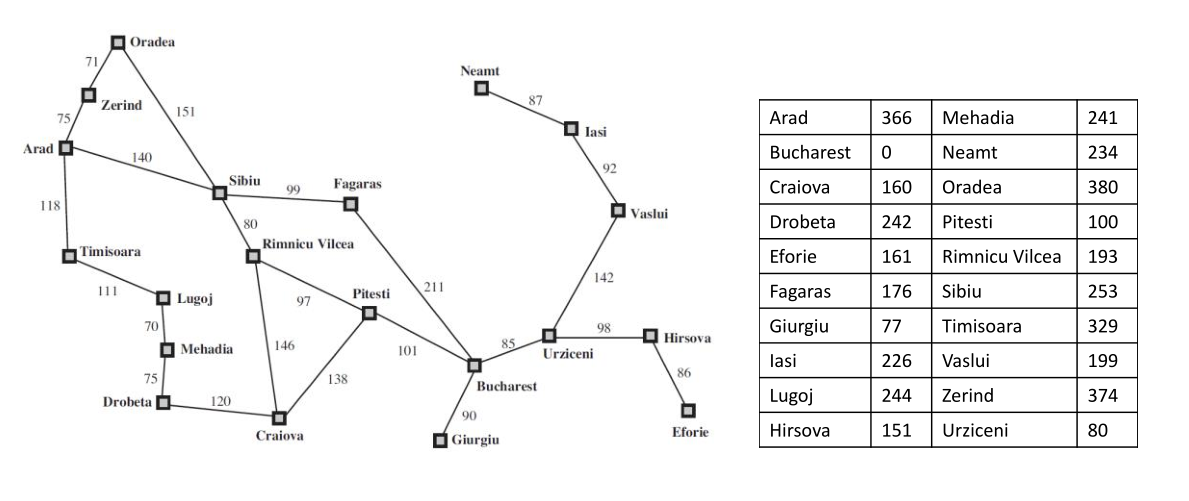
\includegraphics[width=6cm]{images/fig01.png}
	\end{center}
		
		
	\section{Redes Neurais Artificiais}
	
	\item Desenvolva um perceptron que implemente a porta NAND.
	
	\item Explique por quê o Perceptron pode executar as funções lógicas AND, OR e NOT, mas não resolve o OU-EXCLUSIVO (XOR).
	
	\section{Computação Natural}
	
	\item O grafo abaixo mostra a ligação entre 5 cidades e as respectivas distâncias em quilômetros:
	
	\begin{center}
		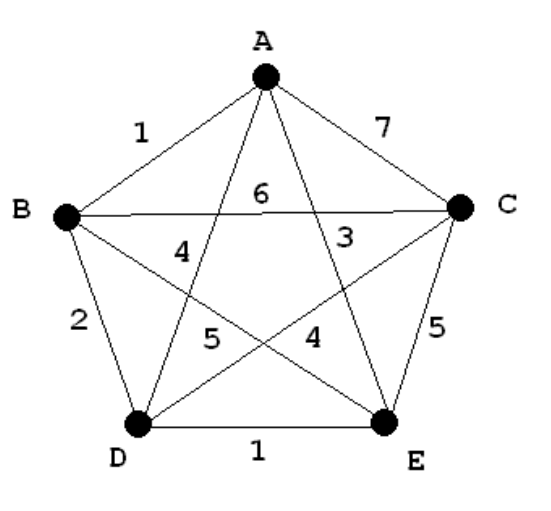
\includegraphics[width=12cm]{images/fig02.png}
	\end{center}
	
	Tem-se um problema em que é necessário passar por todas as cidades, apenas uma vez. O objetivo é encontrar uma rota de menor custo usando um algoritmo genético.
	
	\begin{enumerate}
		\item Proponha uma maneira de codificar os cromossomos.
		\item Defina uma função de aptidão para avaliar a qualidade dos cromossomos.
		\item Gere dois cromossomos e avalie a aptidão deles.
		\item Realize o cruzamento entre os cromossomos.
		\item Aplique uma mutação em um gene dos cromossomos.
		\item Aplique a função de aptidão nos descendentes gerados verificando se a solução encontrada é melhor ou não.
	\end{enumerate}
	
	\newpage
	
	\item Considere a seguinte equação:
	\begin{center}
		$5x + y^2 + w + z^3 = 185$
	\end{center}
	\begin{enumerate}
		\item Proponha uma maneira de codificar os cromossomos.
		\item Defina uma função de aptidão para avaliar a qualidade dos cromossomos.
		\item Defina como o método de seleção dos pais será utilizado.
		\item Defina os operadores genéticos de recombinação e mutação.
		\item Gere uma população inicial de 4 cromossomos e avalie a aptidão deles.
		\item Aplique os operadores de recombinação e mutação sobre essa população para gerar uma nova geração, em seguida avalie a aptidão da nova geração. Repita esse processo por 8 gerações ou até que a solução do problema seja encontrada.
	\end{enumerate}
	
\end{enumerate}

\end{document}